\documentclass[serif]{beamer}
\usepackage[orientation=landscape,size=a0,scale=1.4]{beamerposter}
\usepackage{hyperref} %enable hyperlink for urls
\usepackage[font=scriptsize,justification=justified]{caption}

\newcommand\apj{ApJ}
\newcommand\prd{PRD}
\newcommand\nat{Nature}

\usepackage{ragged2e}

\usepackage{amsmath,amssymb,mathtools}

\usepackage{multicol}

% Replacement palatino fonts
% Would set osf here, but see below
% largesc -> make the small-caps an iota larger (so they match the roman miniscules)
% tighter -> adopt pxfonts spacings (to exploit the better kerning) instead of pagella
% upint -> upright integrals (use much less hspace)
% smallerops -> make the sum/product operators more squat and square
% slantedGreek -> loads italic captical math greeks, to match italic capital math latin
% varbb -> use a less ugly though less conventional blackboard bold DISABLED (see below)
\usepackage[largesc,tighter]{newpxtext}
% Switch the Palatino numbers to the gorgeous `old style' ones. This must be done here
% not as a package option or Babel gets sad. Do it *Before* newpxmath to get osf numbers in maths.
\useosf
\usepackage[upint,smallerops,slantedGreek]{newpxmath}
% Better typewriter font (mono makes it a proper TT font -- currently unsupported though!); 0.9 scales it to the px sizes.
\usepackage[scaled=0.9]{inconsolata}
% Pretty mathcal font, scaled down v. slightly (+ load a decent mathscr font, switch the slightly better looking esstix frakturs and the inordinately better txof bbold)
\usepackage[cal=rsfso,calscaled=.96,scr=rsfs,scrscaled=.96,frak=esstix,frakscaled=.98,bb=txof,bbscaled=1.05]{mathalfa}

\renewcommand\rmdefault{pplx}
\renewcommand\mathfamilydefault{cmr}

\setbeamertemplate{bibliography item}{\insertbiblabel}

\setbeamertemplate{caption}[numbered]
%\setbeamertemplate{enumerate}[circle]
\setbeamertemplate{items}[circle]

\definecolor{ETH1}{RGB}{31,64,122}
\definecolor{ETH3}{RGB}{0,105,180}
\definecolor{ETH6}{RGB}{111,111,110}
\definecolor{ETH8}{RGB}{0,122,146}
\definecolor{ETH10}{RGB}{130,190,30}
\definecolor{tlg}{RGB}{230,230,230}

%%%%%%%%%%%%%%%%%%%%%%%%%%%%%%%%%%%%%%%%%%%%%%%%%%%%%%%%%%%%%%%%%%%%%%%%%%%%%%%%%%%%%%%%%%%%%%%%%%%%
%It seems many of the following entries do not control any visible Behaviour. All such entries are
%set to red, so that they are easy to spot if they ever become visible

\setbeamercolor{headline}{fg=red,bg=white} % This is the recommended color for Specialist community usage: change to ETH1 for general communication
\setbeamercolor{footline}{fg=red, bg=red}
\setbeamerfont{footline}{size=\large,series=\bf}
\setbeamercolor{separation line}{bg=ETH6}
\setbeamercolor{title in headline}{fg=ETH3}
\setbeamercolor{author in headline}{fg=ETH3}
\setbeamercolor{institute in headline}{fg=ETH3}

\setbeamercolor{framesubtitle}{fg=red, bg=ta2gray}
\setbeamercolor{author in head/foot}{fg=ETH3, bg=white}
\setbeamercolor{title in head/foot}{fg=red, bg=red}

\setbeamercolor*{normal text}{fg=ETH6, bg=white}
\setbeamercolor*{block body}{fg=black, bg=white}
\setbeamercolor*{block title}{fg=white,bg=ETH3}
\setbeamerfont{block title}{size=\large,series=\bf}
\setbeamercolor{upper separation line head}{fg=red}

\setbeamercolor*{example body}{fg=red,bg=red}
\setbeamercolor*{example text}{fg=red,bg=red}
\setbeamercolor*{example title}{bg=red,fg=red}

\setbeamercolor{alerted text}{fg=red}
\setbeamercolor{structure}{fg=black}

%\setbeamercolor{itemize item}{fg=ETH3}
%\setbeamertemplate{items}[square]
%\setbeamertemplate{itemize items}{\color{ETH3}$\blacktriangleright$}
\setbeamertemplate{navigation symbols}{}  % no navigation on a poster

\setbeamertemplate{headline}{
	\leavevmode
	\begin{beamercolorbox}[wd=\paperwidth]{headline}
		\vspace{2ex}
		\begin{columns}[c]
			\begin{column}{.09\paperwidth}
			\end{column}
			\begin{column}{.675\paperwidth}
				\raggedleft
				\usebeamercolor{title in headline}{\color{fg}\textbf{\LARGE{\inserttitle}}\\[1ex]}
				\usebeamercolor{author in headline}{\color{fg}\large{\insertauthor}\\[1ex]}
				\usebeamercolor{institute in headline}{\color{fg}\small{\insertinstitute}}
			\end{column}
			\begin{column}{.25\paperwidth}
				\begin{center}
					
\includegraphics[width=.8\textwidth, height=.3\textwidth, keepaspectratio]{Images/RIT2}
				\end{center}
			\end{column}
			\begin{column}{.03\paperwidth}
			\end{column}
		\end{columns}
		\vspace{2ex}
	\end{beamercolorbox}

 	% \begin{beamercolorbox}[wd=\paperwidth]{lower separation line head}
	% 	\rule{0pt}{2pt}
	% \end{beamercolorbox}
	\vskip-2cm
	}

%%%%%%%%%%%%%%%%%%%%%%%%%%%%%%%%%%%%%%%%%%%%%%%%%%%%%%%%%%%%%%%%%%%%%%%%%%%%%%%%%%%%%%%%%%%%%%%%%%%%
\setbeamertemplate{footline}{
	\begin{beamercolorbox}[wd=\paperwidth]{upper separation line foot}
		\rule{0pt}{2pt}
	\end{beamercolorbox}
	\leavevmode%
	\begin{beamercolorbox}[ht=4ex,leftskip=1cm,rightskip=1cm]{author in head/foot}%
        Aasim Zahoor (RIT)
		\hfill
		September 15th, 2020
        \hfill
        \href{https://dcc.ligo.org/LIGO-G1802119}{LIGO-G1802119}
		\hfill
		Aasim.jan@ligo.org
		\vskip1ex
	\end{beamercolorbox}
	\vskip0pt%
	\begin{beamercolorbox}[wd=\paperwidth]{lower separation line foot}
		\rule{0pt}{2pt}
	\end{beamercolorbox}
	}


%\input{paper_submodules/O2RandPPaper/rates_macros.tex}
%\input{paper_submodules/O2RandPPaper/SDDR_macros.tex}
%input{paper_submodules/O2RandPPaper/pe_macros.tex}

%% Units and common defs
\def\Msol{\ensuremath{\mathit{M_\odot}}}
\newcommand\unit[1]{{\rm #1}}

% Parameters
\def\mchirp{\ensuremath{\mathcal{M}_c}{}}
\def\chieff{\ensuremath{\chi_{\textrm{eff}}}{}}
\def\chip{\ensuremath{\chi_p}{}}

\def\mmax{\ensuremath{m_{\textrm{max}}}{}}
\def\mmin{\ensuremath{m_{\textrm{min}}}{}}
\def\mtotmax{\ensuremath{M_{\textrm{max}}}{}}

\def\rater{\ensuremath{\mathcal{R}}{}}
\def\Vc{\ensuremath{V_c}{}}
\def\VT{\ensuremath{\langle VT \rangle}{}}

% commands - \SI{number}{units}  or \si{units}
\newcommand{\SI}[2]{\ensuremath{#1\,{\rm #2}}{}}
\newcommand{\si}[1]{\ensuremath{\rm #1}{}}
\newcommand{\intrv}[3]{\ensuremath{#1_{-#2}^{+#3}}{}}

\def\invstvol{Gpc$^{-3}$ yr$^{-1}$}



\title{
%
  Assessing and marginalizing over CBC waveform systematics with RIFT
%
}
\author{
%
Aasim Jan, Anjali Yelikar and Richard O'Shaughnessy                      %
%
}
\institute{}
\date{September 15th, 2020}


\begin{document}
\begin{frame}{}

\begin{columns}

\begin{column}[T]{.3\textwidth}

\begin{block}{Introduction}
 % The LIGO and Virgo instruments have detected ten black
  %hole binaries in the first two observing runs \cite{o2catalog}.
  Parameter estimation of Gravitational Wave signals a key part of Gravitational Wave Astronomy and Astrophysics. Unbiased and Reliable parameter estimation help achieve a higher precision for tests of General Relativity. Waveforms used to perform parameter estimation produces systematic biases. The goal here is to reasses and mitigate these biases using RIFT.
%  \begin{center}
 %  \begin{columns}
   %   \begin{column}[c]{0.45\textwidth}
      %  \centering
        %\includegraphics[width=\textwidth]{paper_submodules/cbc-catalog/figures/m1_m2_90pc.pdf}
      %\end{column}
      %~
      %begin{column}[c]{0.45\textwidth}
        %\centering
        %\includegraphics[width=\textwidth]{paper_submodules/cbc-catalog/figures/q_chieff_low_high}
      %\end{column}
    %\end{columns}
    %\includegraphics[width=\textwidth]{paper_submodules/cbc-catalog/figures/event_legend_all_ncol6}
    %\vspace{-6.5em}

  %\end{center}

  %emph{
    %\footnotesize
    %Figure: Mass and spin parameter estimates on the ten detected BBH's
    %and one BNS.

    %The BNS is not considered in this analysis.
 % }

  %\vspace{1em}

  %e use these observations to place constraints on the astrophysical
  %distribution of black hole binary masses, spins, and redshifts \cite{LIGO-O2-Rates}.


\end{block}

\vspace{1em}

\begin{block}{RIFT}
Stands for:
\textbf{R}apid parameter inference on Gravitational wave sources via \textbf{I}terative \textbf{F}i\textbf{T}ing
\begin{center}
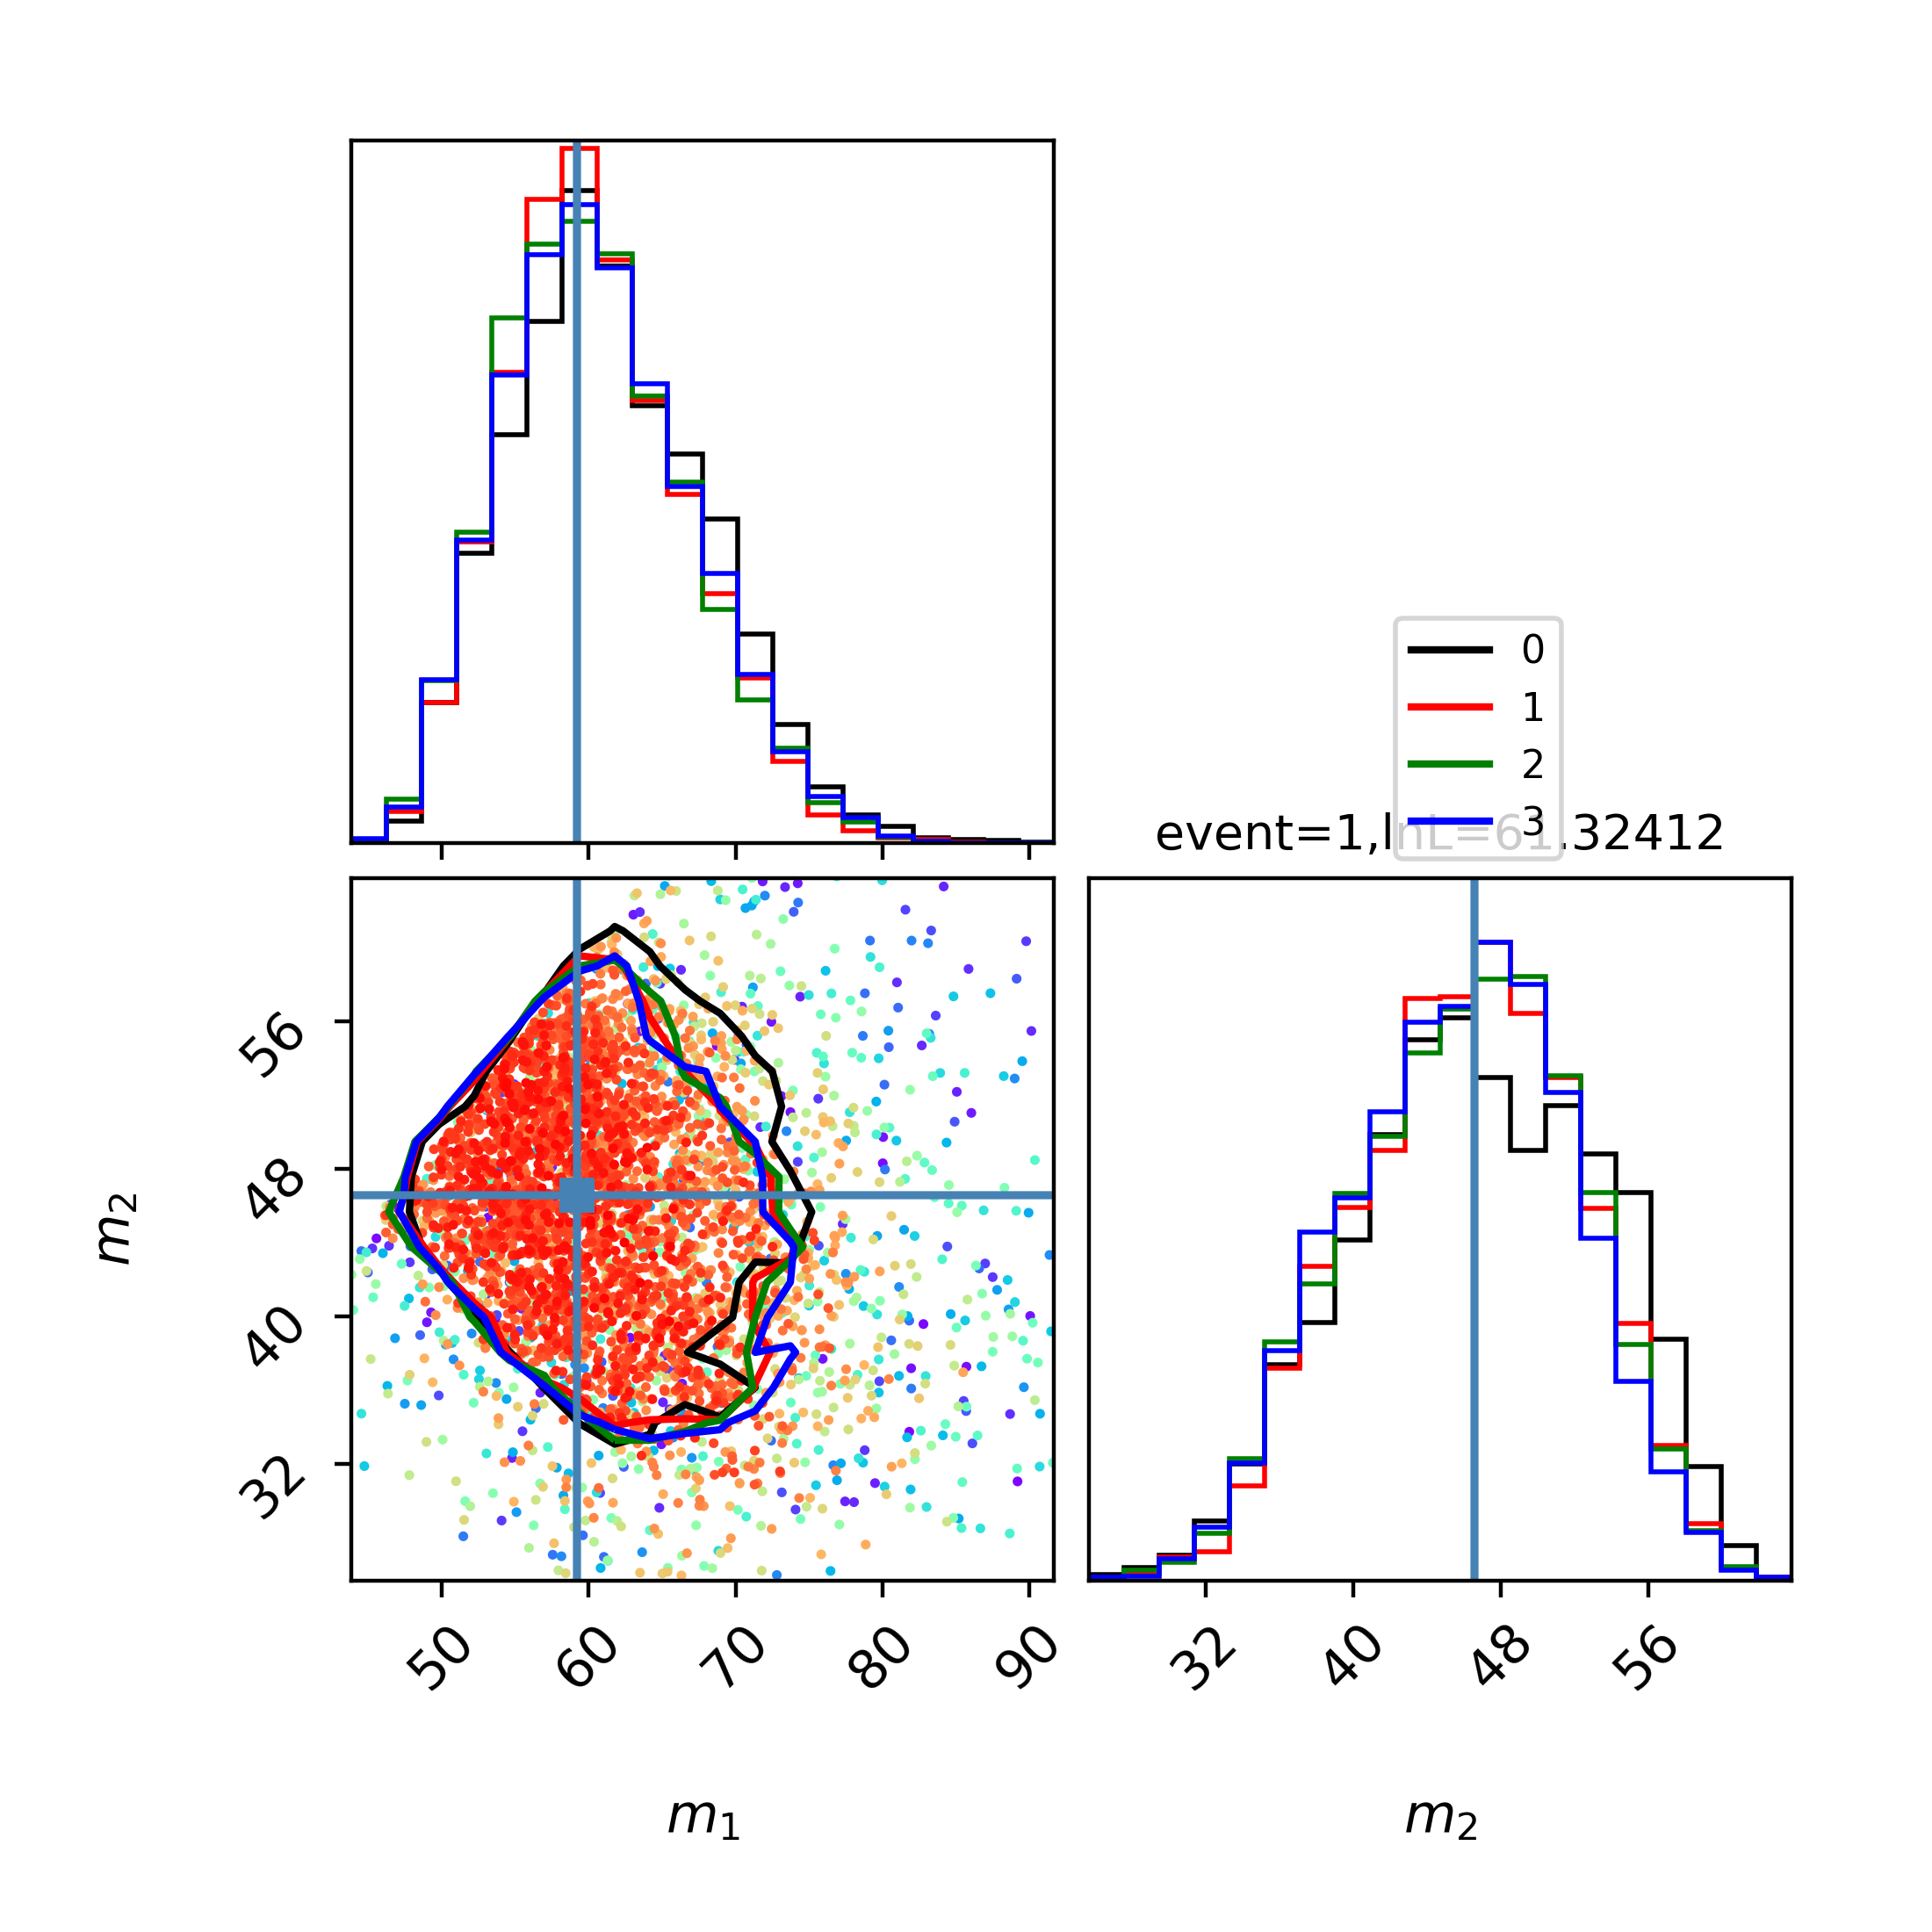
\includegraphics[scale=1.75]{Images/corner_m1_m2}
\end{center}

Based on highly paralleizable grid based parameter estimation strategy. Uses gaussian process interpolation on an unstructured grid.



\end{block}



\end{column}
~
\begin{column}[T]{0.35\textwidth}

\begin{block}{PP plots}
X axis is the probability contained in a credible interval and on the y axis the fraction of true values which lay inside that interval.


  \begin{center}
    \begin{columns}
      \begin{column}{0.45\textwidth}
        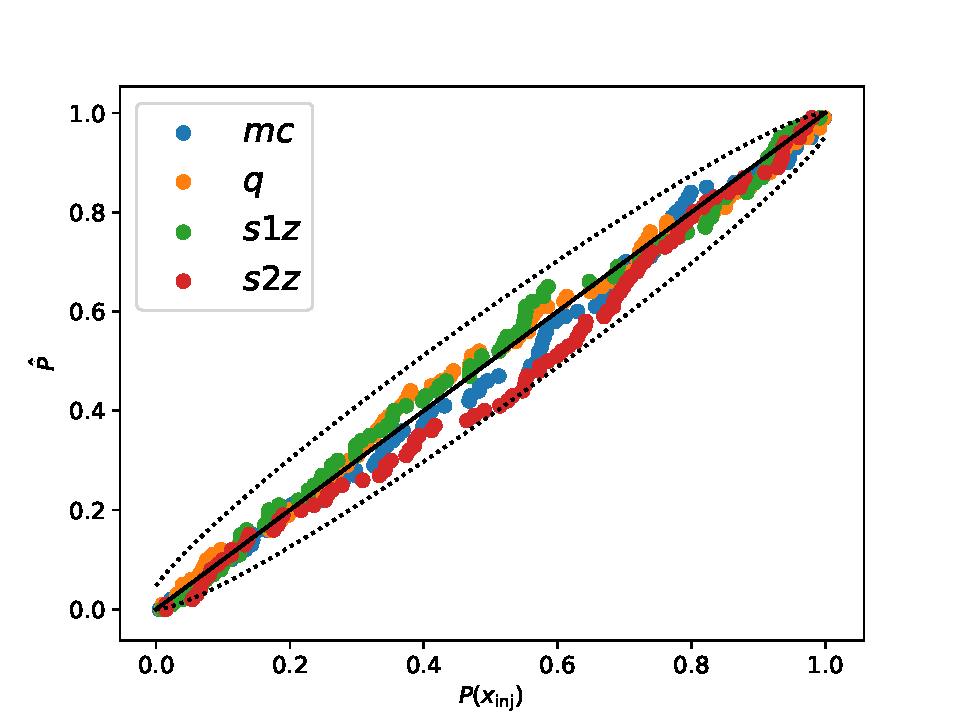
\includegraphics[width=\textwidth]{Images/pp_plot_SEOB}
      \end{column}
      ~
      \begin{column}{0.45\textwidth}
        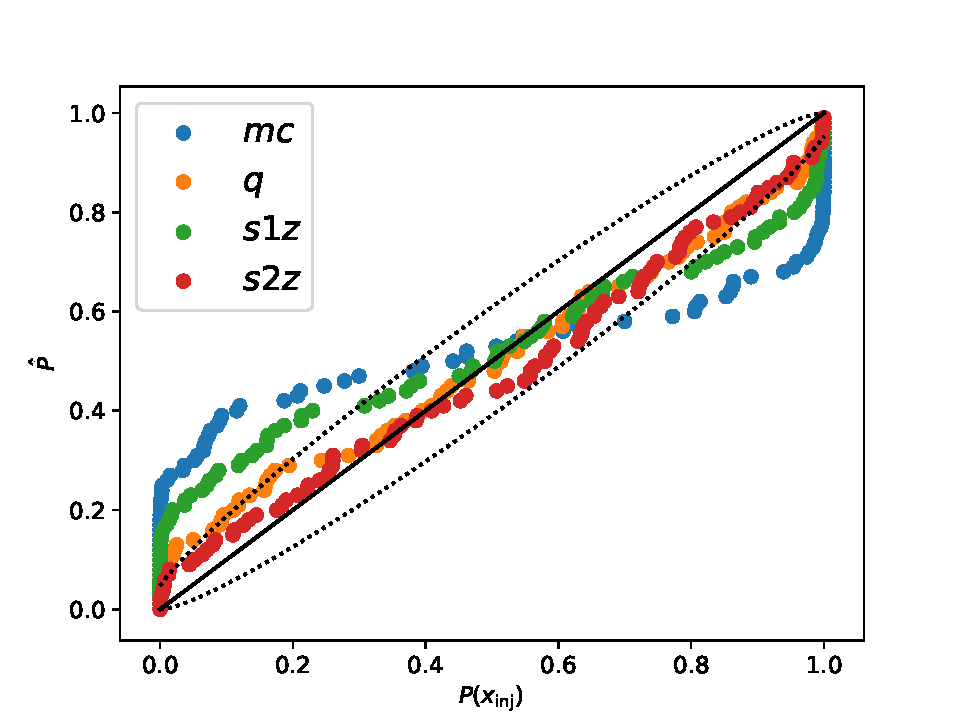
\includegraphics[width=\textwidth]{Images/pp_plot_IMRD}
      \end{column}
    \end{columns}
   \includegraphics[scale=1.5]{Images/Sample_vectorplot}
   \end{center}
  \vspace{-3.5em}


%\noindent \emph{Rate, mass distribution, and spin distribution correlated}: Joint inference! Strong correlation between mass
  %distribution features and merger rate.

\end{block}

%% \begin{block}{Parameter Constraints}
%%  key ideas:

%% - basic rate-shape correlation

%% - minimum mass not being informative.
%%       (Possibly show minimum mass down to 3 Msun as extra option?)
%% \end{block}

\vspace{1em}

\begin{block}{Model Marginalisation}





\end{block}


\vfill
\end{column}
~
\begin{column}[T]{0.3\textwidth}


\begin{block}{Model Marginalisation Plots}

\end{block}

\vspace{1em}

\begin{block}{Conclusions}


\end{block}

\end{column}

\end{columns}

\vspace{1em}

\begin{block}{References}
\vspace{-1em}
\begin{multicols}{2}
%  {\tiny
  %  \bibliographystyle{abbrv}
    %\bibliography{paper_submodules/O2RandPPaper/references,poster.bib}
  %}

\end{multicols}

% {\tiny
% %  \footnotesize
%   \bibliographystyle{unsrtnat}
%   \bibliography{paper_submodules/O2RandPPaper/references,poster.bib}
% }
\end{block}
\end{frame}
\end{document}



















